\section{Laboratory work implementation}

\subsection{Tasks and Points}

\begin{enumerate}

\item Create a Windows application
\item In the middle of the window should be present the following text: "Done with Pride and Prejudice by student name". Replace student name with your name.
\item On windows resize, text should reflow and be in window's middle (vertically and horizontally).
\item Add 2 buttons to window: one with default styles, one with custom styles (size, background, text color, font family/size).
\item Add 2 text elements to window: one with default styles, one with custom styles (size, background, text color, font family/size).
\item Make elements to interact or change other elements (2 different interactions)  (ex. on button click, change text element color or position).
\item Changed behavior of only one window action due to the fat that I were programming in Android and was overridden only back button functionality

\end{enumerate}
\subsection{Laboratory work analysis}

Link to my GitHub repository : 

\url{https://github.com/Tolea86/WP_ANDROID/tree/master/LAB_1/PW_lab1}\\

My application has following features : it has a text centered in the middle, which re-centers on resize, it has two text views one with default style and one with custom style, it has two buttons one with default style and one with custom style both with actions, clicking on button1 will change the text of text1, clicking on button2 will change the background color of button1 to a random color. Also is overridden the functionality of back button from Android. 

\subsection{Prove your work with screens}

a), b), d), e)

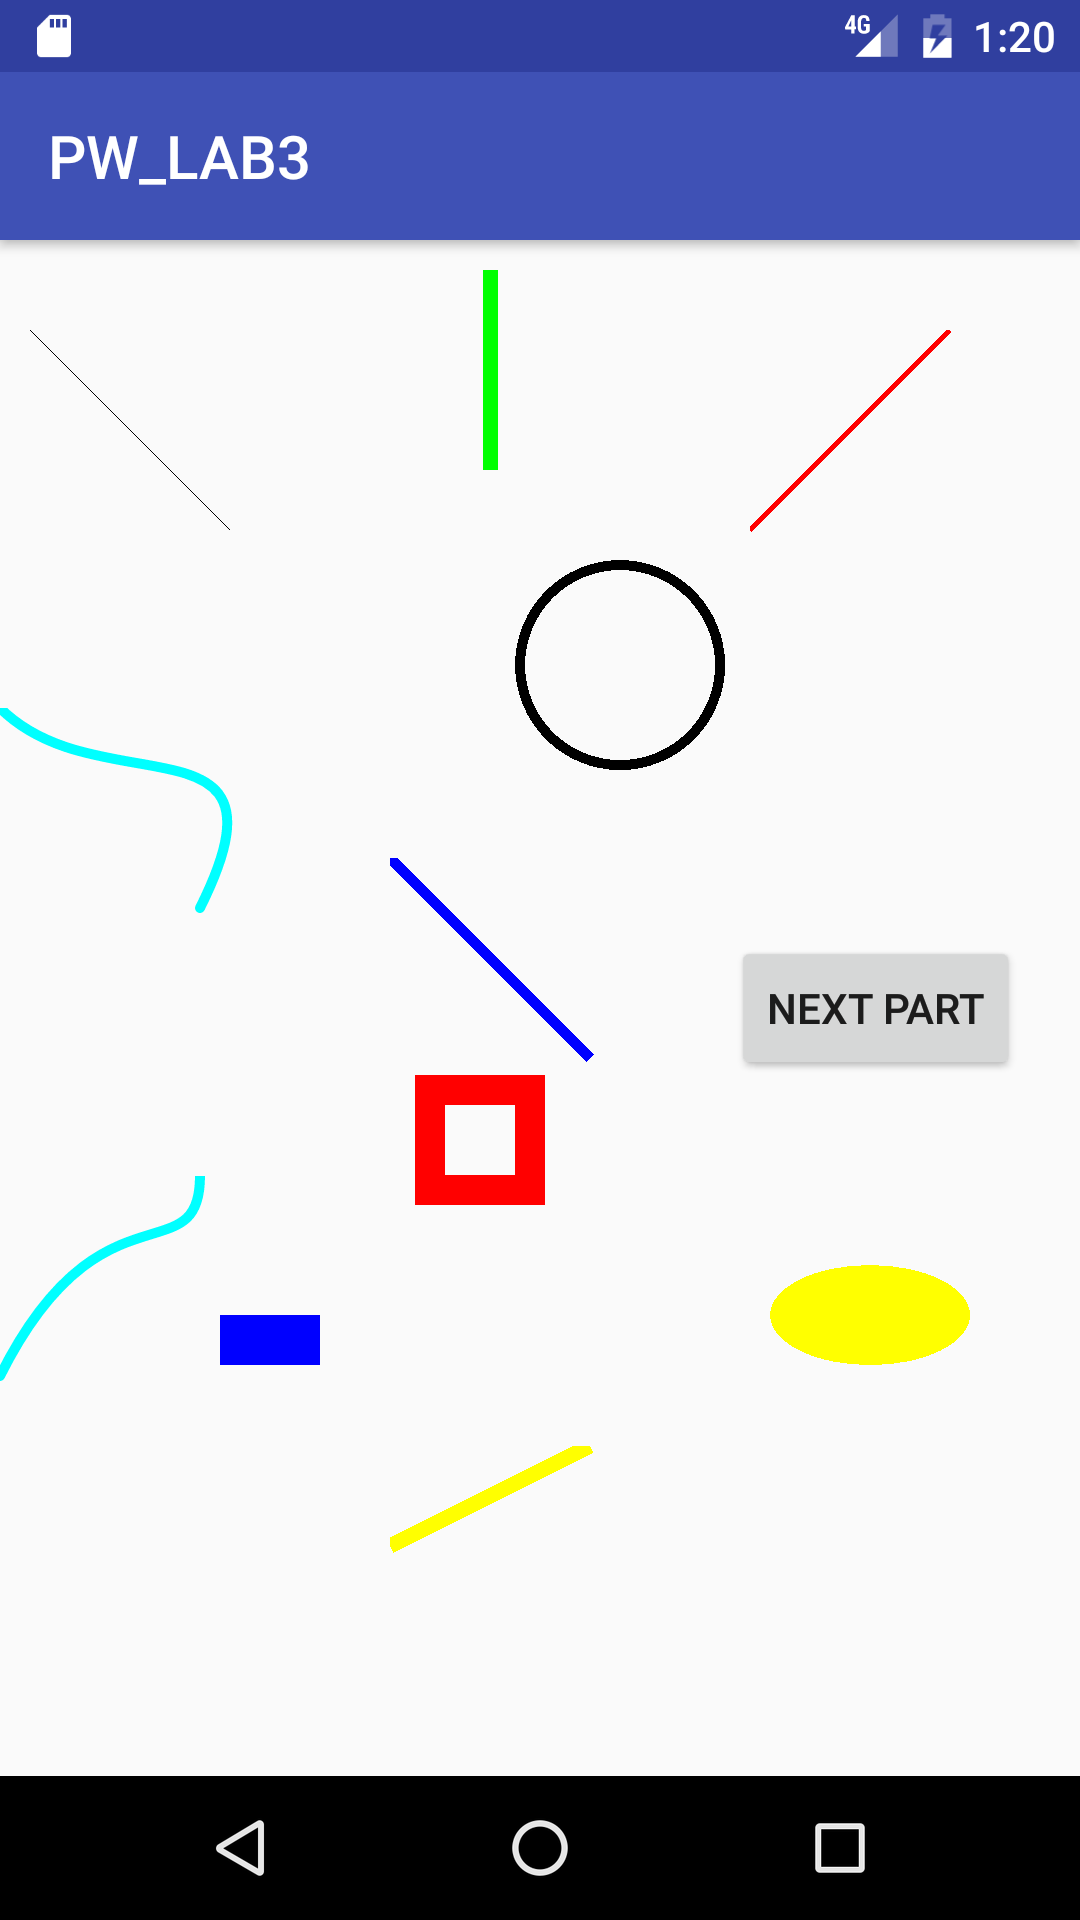
\includegraphics[scale=0.5]{screen1}

c)

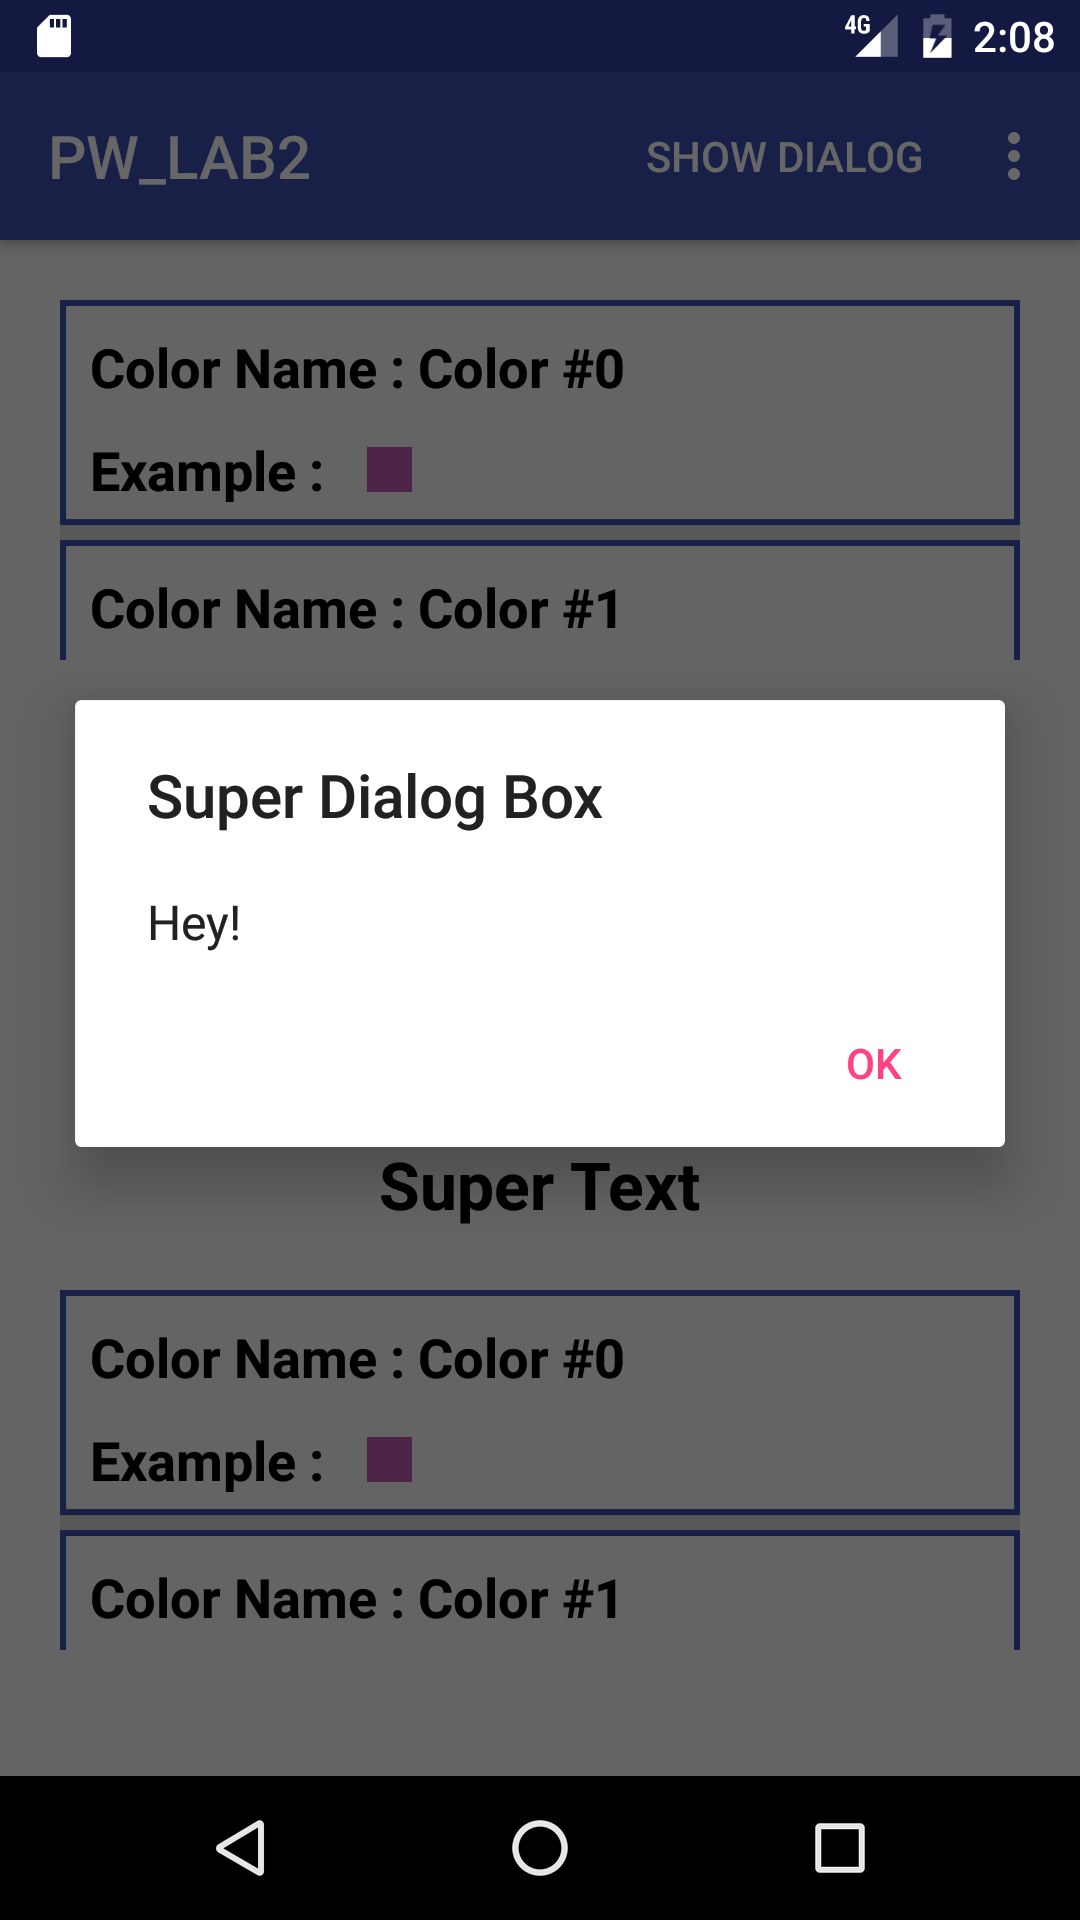
\includegraphics[scale=0.5]{screen2}

f) button1 clicked

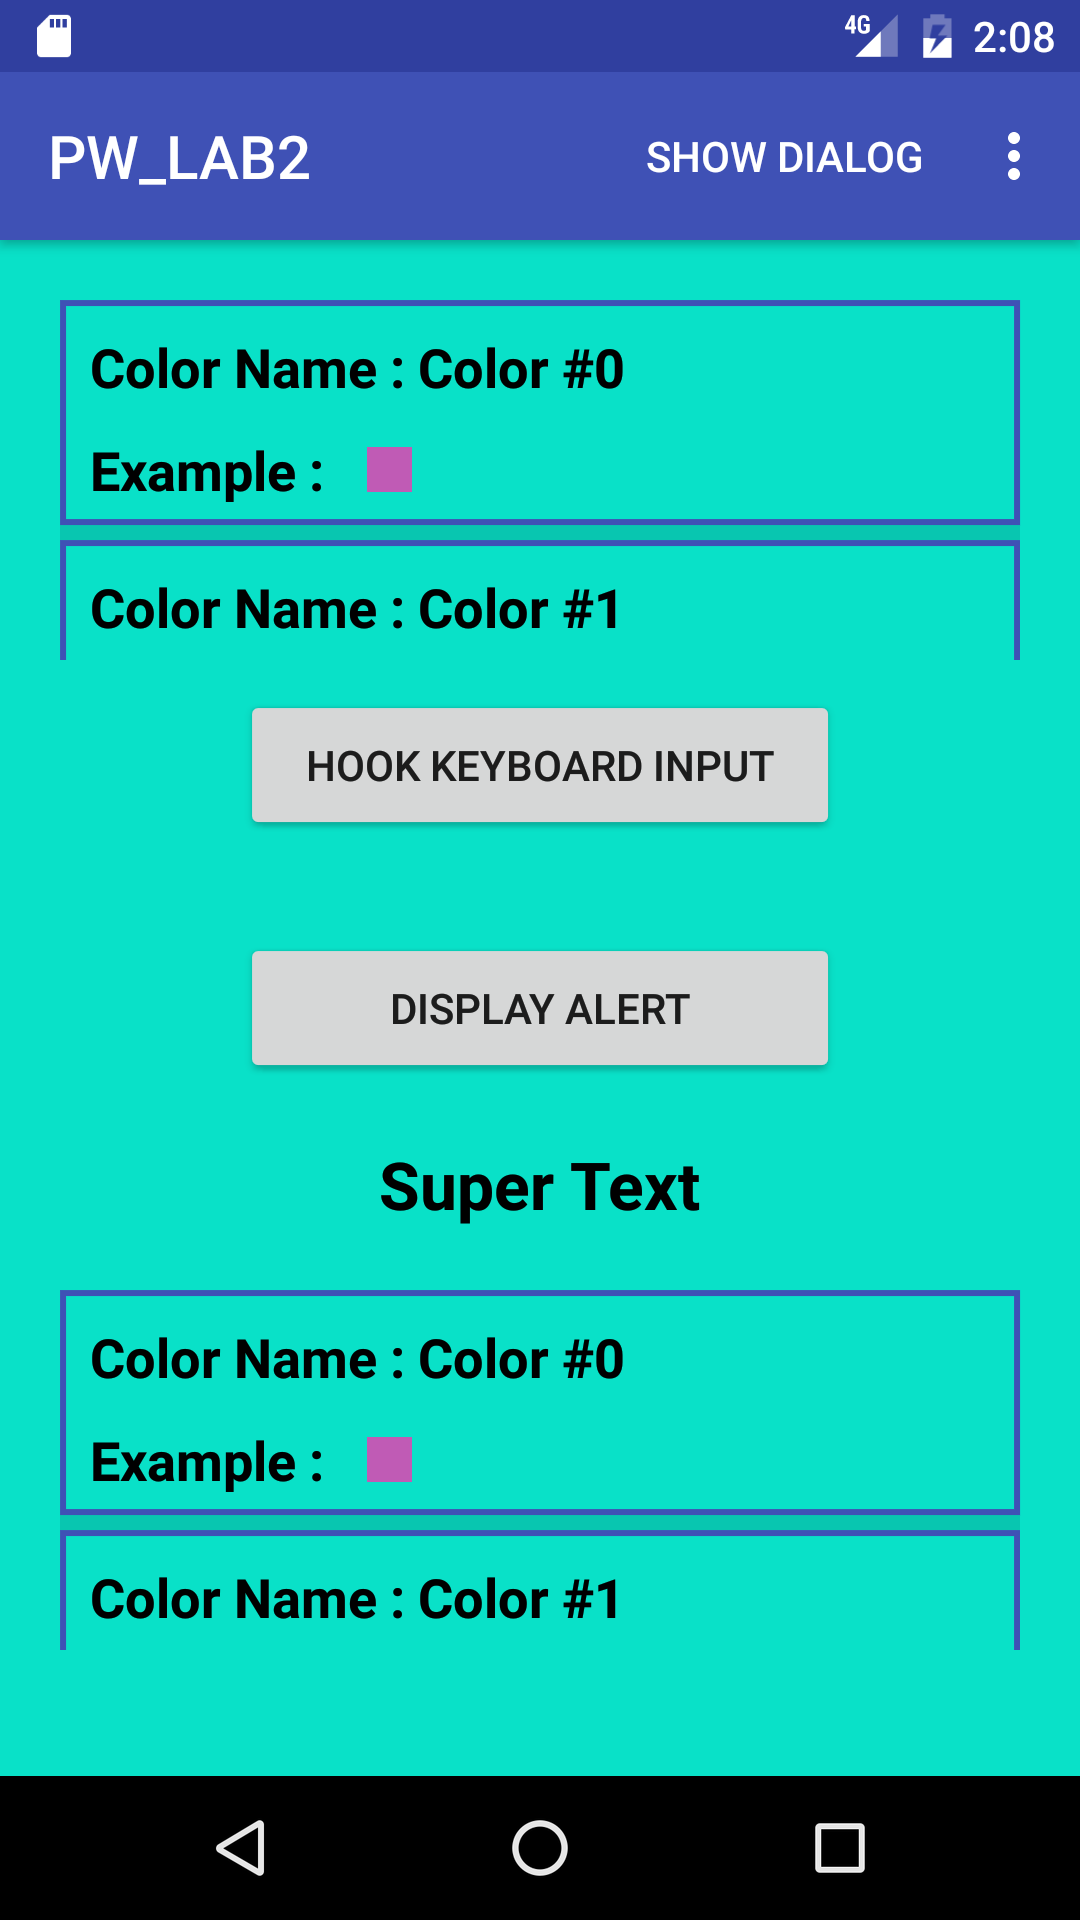
\includegraphics[scale=0.5]{screen3}

f) button2 clicked

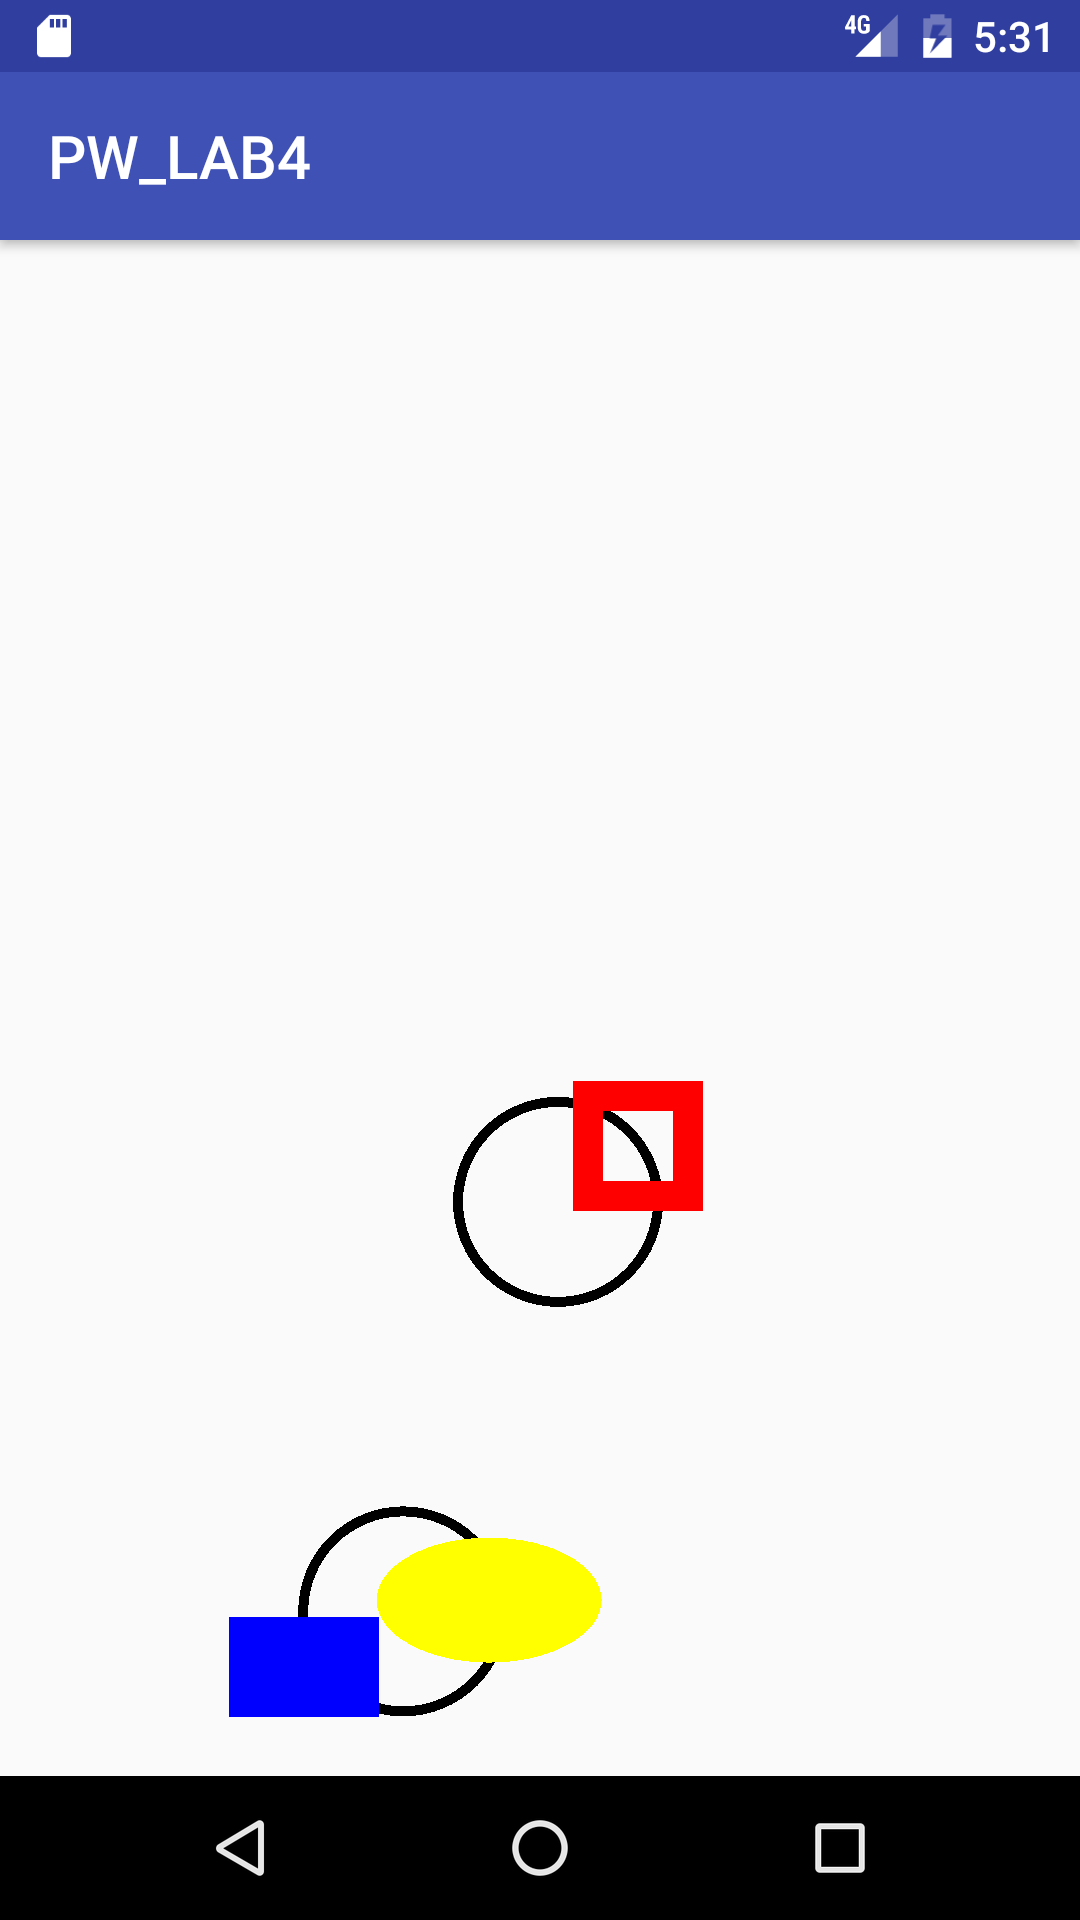
\includegraphics[scale=0.5]{screen4}

g) back button clicked

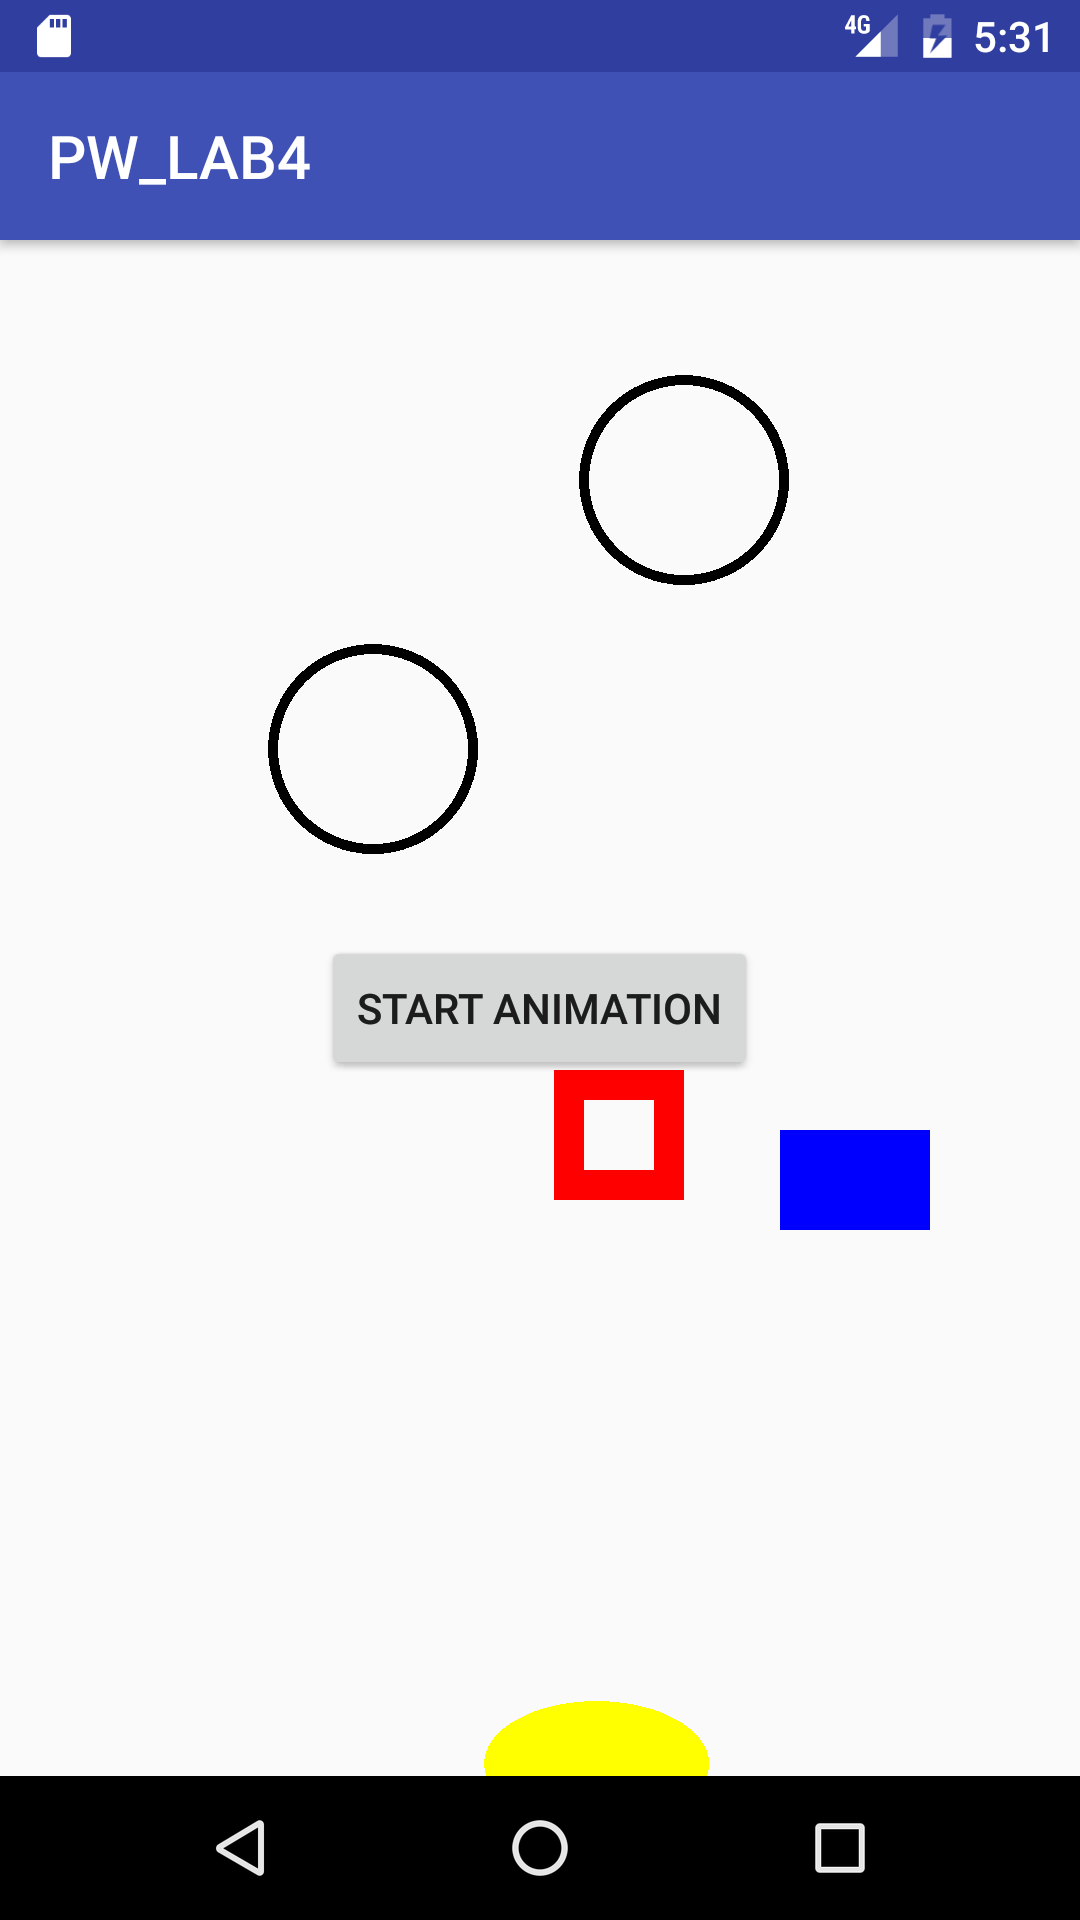
\includegraphics[scale=0.5]{screen5}

\clearpage